\section{Segunda iteración}

En esta segunda iteración pretendemos mejorar algunos de los aspectos que nos hemos encontrando en la primera, o aspectos que simplemente hemos dejado para después. Comenzaremos con una alternativa al balanceo de datos, y luego probaremos otros tipos tanto de aprendizaje como de modelos.

\subsection{Balanceo de datos}\ \label{sec:i2-balance}

La toma de nuevos datos es costosa y como tenemos relativamente pocos para la cantidad de columnas (las 168 longitudes de onda), el balanceo de datos es esencial. En la primera iteración, intentamos sortear este problema utilizando métricas que tienen en cuenta el balance de los datos. Sin embargo, podemos balancear los datos en dos pasos: \textit{undersampling} y \textit{oversampling}. 

Como su nombre indica, \textit{undersampling} es una técnica para reducir las muestras de la clase mayoritaria, en nuestro caso los granos sin contaminar. Existen varias técnicas para hacer \textit{undersampling}, las cuales comentaremos en la \textit{sección\ \ref{sec:undersampling}}. Por otro lado, el \textit{oversampling} consiste en la creación de datos sintéticos, similares a los reales, para suplir la diferencia de granos. Al igual que con el \textit{undersampling}, existen diversas técnicas que comentaremos más adelante en la \textit{sección\ \ref{sec:oversampling}}.


\subsubsection{\textit{Undersampling}}\ \label{sec:undersampling}

A la hora de balancear los datos, buscamos, de alguna forma, reducir la diferencia en el número de muestras en las diferentes clases. En el paso de \textit{undersampling}, buscamos reducir la cantidad de muestras de las clases mayoritarias, recordamos que nuestro caso lo podemos ver en la \textit{figura\ \ref{fig:unbalance}}. Para ello, debemos de alguna forma determinar qué muestras de las clases mayoritarias son más redundantes para evitar eliminar muestras `críticas'. Comentaremos a continuación diferentes algoritmos que nos ayudan con este paso.

Los algoritmos que hemos decidido utilizar son los de la librería \href{https://imbalanced-learn.org/stable/}{imblearn} que fue diseñada específicamente para los problemas de clasificación sobre \textit{datasets} desbalanceados.\ \cite{3Undersa98:online}

El primer algoritmo que probaremos será \textit{RandomUnderSampler}, el cual consiste en seleccionar un subconjunto aleatorio de datos. Para intentar no eliminar datos importantes como hemos comentado antes, aplica una de las tres versiones de la heurística \textit{NearMiss}\ \cite{3Undersa98:online}, la cual se basa en el algoritmo \textit{nearest neighbors}:

\begin{enumerate}
    \item La versión \textbf{1} elimina aquellos datos cuya distancia media a sus \textit{N} vecinos más cercanos de la clase minoritaria sea menor.
    \item La versión \textbf{2} es parecida a la \textbf{1}, pero en esta la distancia media se computa sobre los \textit{N} vecinos más lejanos de la clase minoritaria.
    \item La versión \textbf{3} consta de dos pasos, primero de cada elemento de la clase minoritaria selecciona los \textit{M} vecinos más cercanos de la clase mayoritaria. Luego, por cada muestra seleccionada se calcula la distancia media respecto a los \textit{N} vecinos más cercanos de la clase minoritaria y se eliminan los que, de media, estén más alejados.
\end{enumerate}

El algoritmo \textit{Tomek Links} detecta los llamados \textit{Tomek Links}, estos son enlaces entre dos muestras de diferente clase, pongamos \(x\) e \(y\), definidos tal que para cualquier muestra \(z\): 
\[d(x,y) < d(x,z)\ and\ d(x,y) < d(y,z)\], donde \(d(a, b)\) es la distancia entre la muestra \(a\) y \(b\). En resumen, un \textit{Tomek Link} se da entre las muestras de distintas clases más cercanas entre sí. Este algoritmo suele ser bueno a la hora de eliminar ruido en los datos.

\textit{Edited Nearest Neighbours} en resumen elimina las muestras que no se parezcan demasiado a sus vecinos\ \cite{Wil72}. Para ello, comprueba para cada muestra que sus \textit{N} vecinos más cercanos sean de su misma clase, y si no podemos elegir si nos quedamos con la mayoría o si eliminamos todas las muestras.

\textit{InstanceHardnessThreshold} es un algoritmo que entrena un modelo de \textit{sklearn} sobre los datos y elimina aquellas muestras de las cuales está menos seguro.


\subsubsection{\textit{Oversampling}}\ \label{sec:oversampling}

El segundo paso es el \textit{oversampling}, el cual consiste en la creación de los datos sintéticos para suplir la carencia de datos de una clase minoritaria. Hay algoritmos para realizar estas técnicas implementados en \textit{imblearn}, sin embargo preferimos utilizar \href{https://sdv.dev/}{sdv}, pues tiene mejor documentación y tiene un método `fácil' para evaluar los datos generados. \cite{Synthesi69:online} En general, los sintetizadores utilizan algoritmos complejos sobre los cuales podemos leer en \cite{Synthesi69:online}, pero para agilizar el proceso de análisis no entraremos demasiado en detalle.

Antes de comentar los sintetizadores que probaremos, comentaremos el método de evaluación de los datos generados con los que los evaluaremos. Utilizaremos una función de la propia librería \textit{sdv} que evalúa la similitud estadística de los datos generados con los datos reales.

Los tres sintetizadores que probaremos son:

\begin{enumerate}
    \item \textit{Gaussian Copula Synthesizer} \cite{Gaussian4:online}, el cual utiliza unos métodos clásicos estadísticos.
    \item \textit{CTGANSynthesizer} \cite{CTGANSyn50:online}, utiliza métodos de \textit{deep learning} basados en \textit{GAN} \cite{Generati72:online}.
    \item \textit{TVAESynthesizer} \cite{TVAESynt0:online}, basado en \textit{VAE} \cite{Variatio61:online}, utiliza técnicas de redes neuronales.
\end{enumerate}

#HERE

Para hacer \textit{oversampling} utilizamos la librería \href{https://sdv.dev/}{sdv}, más específicamente el \href{https://docs.sdv.dev/sdv/single-table-data/modeling/synthesizers/gaussiancopulasynthesizer}{GaussianCopulaSynthesizer}, el cual utiliza métodos estadísticos clásicos para generar datos sintéticos parecidos a los reales. Una vez generados los datos sintéticos, podemos comprobar su calidad generando un reporte de calidad de la con la misma librería \textit{sdv}, utilizando la función \href{https://docs.sdv.dev/sdv/single-table-data/evaluation#evaluate_quality}{evaluate\_quality} la cual compara los datos generados con los reales y nos da los resultados de la \textit{figura\ \ref{fig:quality_report}}.

\begin{figure}[!ht]
    \centering
    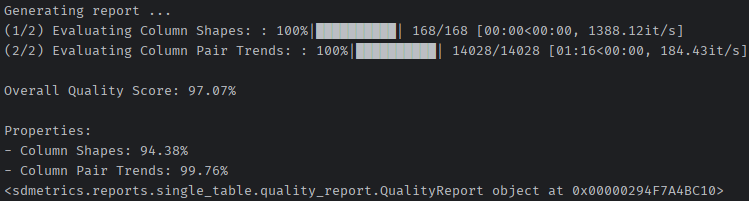
\includegraphics[width=0.8\linewidth]{media/images/quality_report.png}
    \caption{Reporte de calidad de los datos generados sintéticamente, fuente propia.}\ \label{fig:quality_report}
\end{figure}

Una vez aplicados los dos algoritmos obtenemos un \gls{dataset} balanceado como el de la \textit{figura\ \ref{fig:balance}}.

La toma de nuevos datos reales es costosa, y como teníamos relativamente pocos datos para entrenar el balanceo es esencial. Podemos hacer unos entrenamientos y comparar los resultados para ver si es necesario 
balancear, los resultados los podemos ver en la \textit{tabla\ \ref{tab:balanced_comparison}}. Fijándonos en las columnas a partir de \textit{f1score}, ya que estas son las métricas que ignoran el balanceo de 
los datos, podemos ver que, son mejores los modelos entrenados sobre el \gls{dataset} balanceado.

\begin{table}[!ht]
    \centering
    \resizebox{\textwidth}{!}{\begin{tabular}{|c|ccccc|ccccc|} \hline
    & \multicolumn{5}{|c|}{Balanced dataset} & \multicolumn{5}{c|}{Unbalanced dataset} \\ \hline
        Model Name & Train score & Test score & f1score & f0.5score & Balanced accuracy & Train score & Test score & f1score & f0.5score & Balanced accuracy \\ \hline
        XGBoost model & 92.051 & 87.669 & 87.055 & 89.736 & 87.669 & 82 & 82 & 0 & 0 & 50 \\
        Stochastic Gradient Descent & 79.584 & 78.862 & 76.506 & 81.988 & 78.862 & 64.815 & 56.444 & 24.615 & 20.075 & 49.834 \\
        Random Forest model & 94.399 & 87.398 & 86.58 & 90.09 & 87.398 & 99.926 & 87.778 & 49.541 & 69.948 & 66.531 \\
        Quadratic Discriminant Analysis & 87.94 & 87.669 & 86.191 & 92.871 & 87.669 & 96.148 & 83.111 & 54.217 & 53.444 & 72.358 \\
        Multi-Layer Perceptron & 89.205 & 85.908 & 85.014 & 88.376 & 85.908 & 90.815 & 84 & 32.075 & 46.961 & 59.41 \\
        Linear Discriminant Analysis & 82.746 & 80.759 & 78.743 & 84.026 & 80.759 & 85.333 & 78.222 & 20.968 & 25.692 & 53.96 \\
        LightGBM model & 92.141 & 87.127 & 86.409 & 89.402 & 87.127 & 82.222 & 72.222 & 48.133 & 40.222 & 71.981 \\
        K-Neighbors model & 100 & 83.333 & 81.048 & 88.314 & 83.333 & 100 & 86.889 & 55.639 & 64.014 & 70.807 \\
        Hist Gradient Boosting model & 82.294 & 81.436 & 79.764 & 84.322 & 81.436 & 78.444 & 70.444 & 44.813 & 37.448 & 68.97 \\
        Extra Trees model & 86.224 & 84.688 & 82.695 & 89.701 & 84.688 & 99.63 & 90.444 & 69.504 & 76.324 & 78.756 \\
        Decision Tree model & 80.352 & 79.268 & 76.279 & 83.503 & 79.268 & 56.963 & 58.889 & 41.27 & 31.957 & 67.224 \\ \hline
    \end{tabular}}
    \caption{Tabla comparativa de los resultados de entrenar los modelos con los datos balanceados y sin balancear, después de preprocesar los datos. Fuente propia.}\ \label{tab:balanced_comparison}
\end{table}


\begin{figure}[!ht]
    \centering
    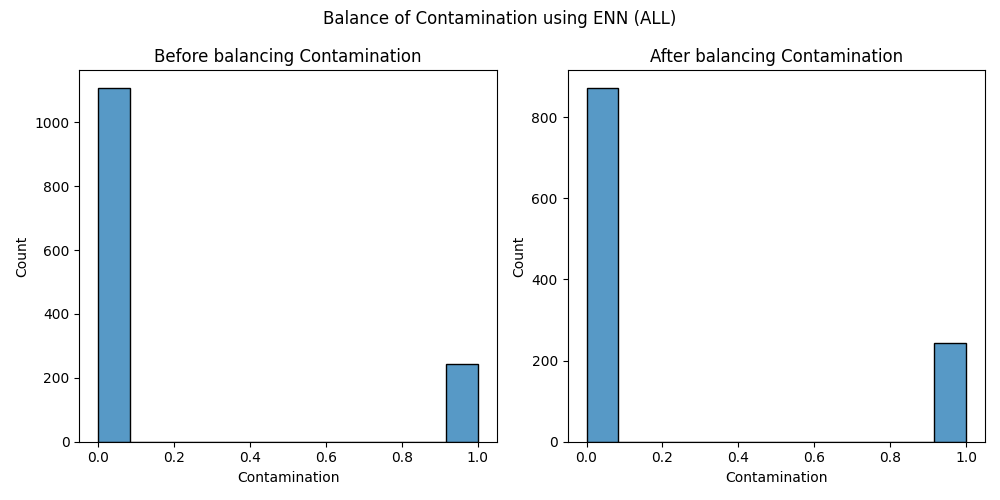
\includegraphics[width=0.6\linewidth]{media/images/balance.png}
    \caption{Comparación del balanceo de la clase objetivo del \gls{dataset} antes y después de balancear, fuente propia, código\ \ref{code:plots_balancing}}\ \label{fig:balance}
\end{figure}